 %!TEX root=title.tex
\section{Social Weaver Analysis}
\subsection{Social Weaver in Action}
This chapter leads us through an real example where Social Weaver is being used. It is explained which components are used in what situations and how they interact with each other. Again we use Google Calendar as basis for the scenario.

\subsubsection{Google Calendar}
Google Calendar\footnote{\url{http://google.com/calendar}} (GCal) is free service for time management or in other words an electronic calendar (see Figure \ref{gcal-plain}). In the following context GCal describes the web application, that is accessible with any browser. The particular reason why we use GCal as testing scenario, is that it is a freely available web application with shared data across user sessions. Such data can be a single appointment or a entirely shared calendar. Even though the HTML code differs for such data, the equality is clear to the user.

\subsubsection{Challenges}
The challenges with GCal is the differing HTML code for equally elements across user sessions. Consider the following code for an appointment:

\begin{lstlisting}[language=HTML]
<div class="ca-evp7 chip" style="top:252px;left:-1px;width:100%;">
	<dl class="cbrd" style="height:35px;border-color:#9FC6E7;background-color:#E4EFF8;color:#777777;">
		<dt style="background-color:;">
			06:00 - 07:00
			<i class="cic cic-dm cic-prsn" title="Guests"> </i>
		</dt>
		<dd>
			<span class="evt-lk ca-elp7" style="cursor: pointer;">Alice and Bob Meeting</span>
		</dd>
		<div>
			<div class="mask mask-top" style="border-color:#9FC6E7;background-color:#E4EFF8;"> </div>
			<div class="mask mask-bottom" style="border-color:#9FC6E7;background-color:#E4EFF8;"> </div>
			<div class="mask mask-left" style="height:38px;border-color:#9FC6E7;background-color:#E4EFF8;"> </div>
			<div class="mask mask-right" style="height:38px;border-color:#9FC6E7;background-color:#E4EFF8;"> </div>
		</div>
		<div class="resizer">
			<div class="rszr-icon"> </div>
		</div>
	</dl>
</div>
\end{lstlisting}

At a first glance the \verb+span class="evt-lk ca-elp7"+ seems to be a unique identifier for an appointment, but unfortunately in a different session the shared appointment have \verb+span class="evt-lk ca-elp6"+. For that reason we need to use the same information that the users uses to determine the appointment. This information is time, date and title. Unless the users are in different time zones, these parameters are reliable. (Time zone support is possible but not noticed in the thesis.)

\begin{figure}\centering
	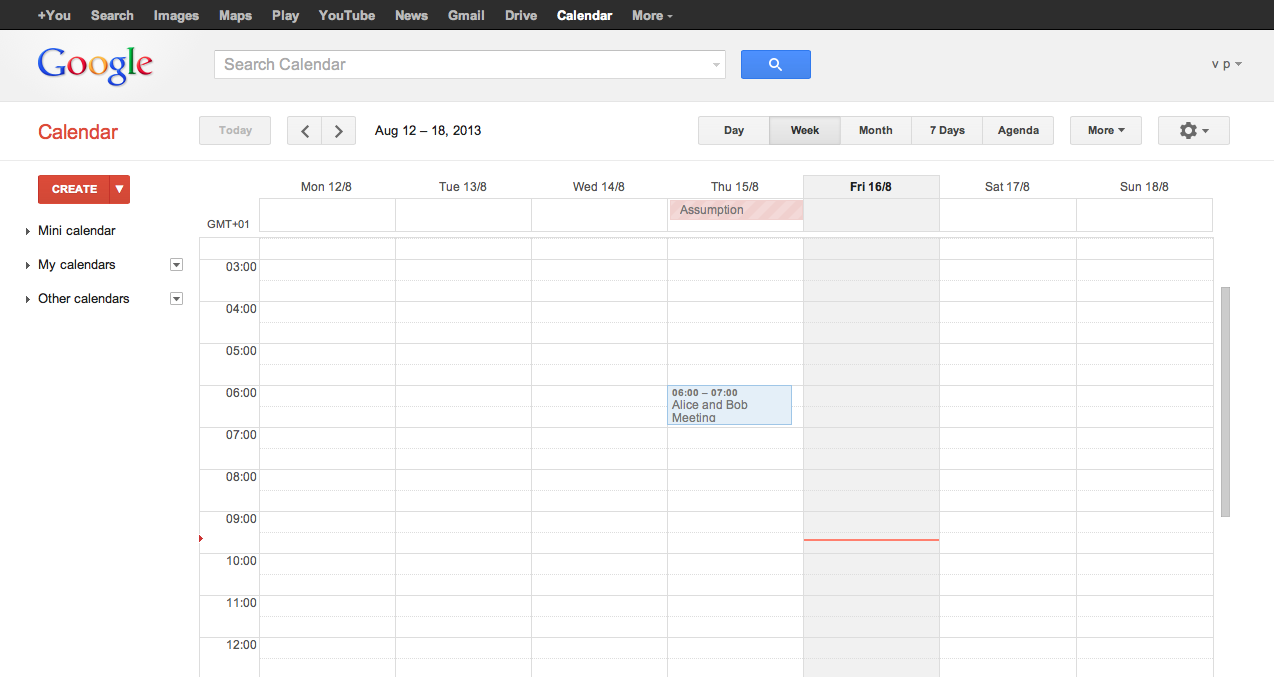
\includegraphics[width=10cm]{images/gcal-plain.png}
\caption{Initial situation in Google Calendar}
\label{gcal-plain}
\end{figure}

\subsubsection{Initial Scenario}
The following explanations are based on a scenario with two users (Alice and Bob) who both are running the Social Weaver plugin in Firefox and are connected to the same Web Service (which means they share the same Social Weaver session). 

Additionally they obviously need a shared Google calendar. For accessing the calendar they use the default web service provided by Google and no alternative client. 

The scenario consists of the following steps:
\begin{enumerate}
	\item Alice weaves a comment box to an appointment in the shared calendar
	\item Alice uses the comment box to leaves a reminder
	\item Bob logs in and comments Alice's reminder 
	\item We manually destroy the anchor directly in the database
	\item Alice recognizes this failure and re-links the comment box
\end{enumerate}

In the following two sub-procedures, update and matching, are explained. The reason why we handle those separately is, that we use them more frequently in the whole process. That way we can just refer to them and keep the focus on the actual work-flow. 

\subsubsection{Update Procedure}
The synchronization for Social Weaver is quite simple. Basically, the plugin sends at start up (or when asked) two parameters in a JSON array to the web service using a authenticated POST request. Those parameters are the current URL and the time stamp of the last update. If Alice starts up her first browser the first time, the plugin would send the following JSON file:

% TODO nochmal pruefen

\begin{lstlisting}[language=JavaScript]
{
	last_update=1376640808,
	current_url='http://google.com/calendar'
}
\end{lstlisting}

The web service uses those information to determine whether there are new and relevant anchors or not. In the positive case (see Figure \ref{sequence-update}) the anchors are returned. In Alice's case nothing is returned since we have no marked elements. 

What happens at the server with those data in detail? We use the time stamp of the last update and the current URL to create a query that receives only the corresponding anchors. 

Through a simple HTTP header authentication we know which user is getting access to the anchor data. Even though it is not really relevant in our simple case. It would be more an issue when having multiple users in different session in one Social Weaver context. But such scenarios aren't covered in this thesis.

\begin{figure}\centering
		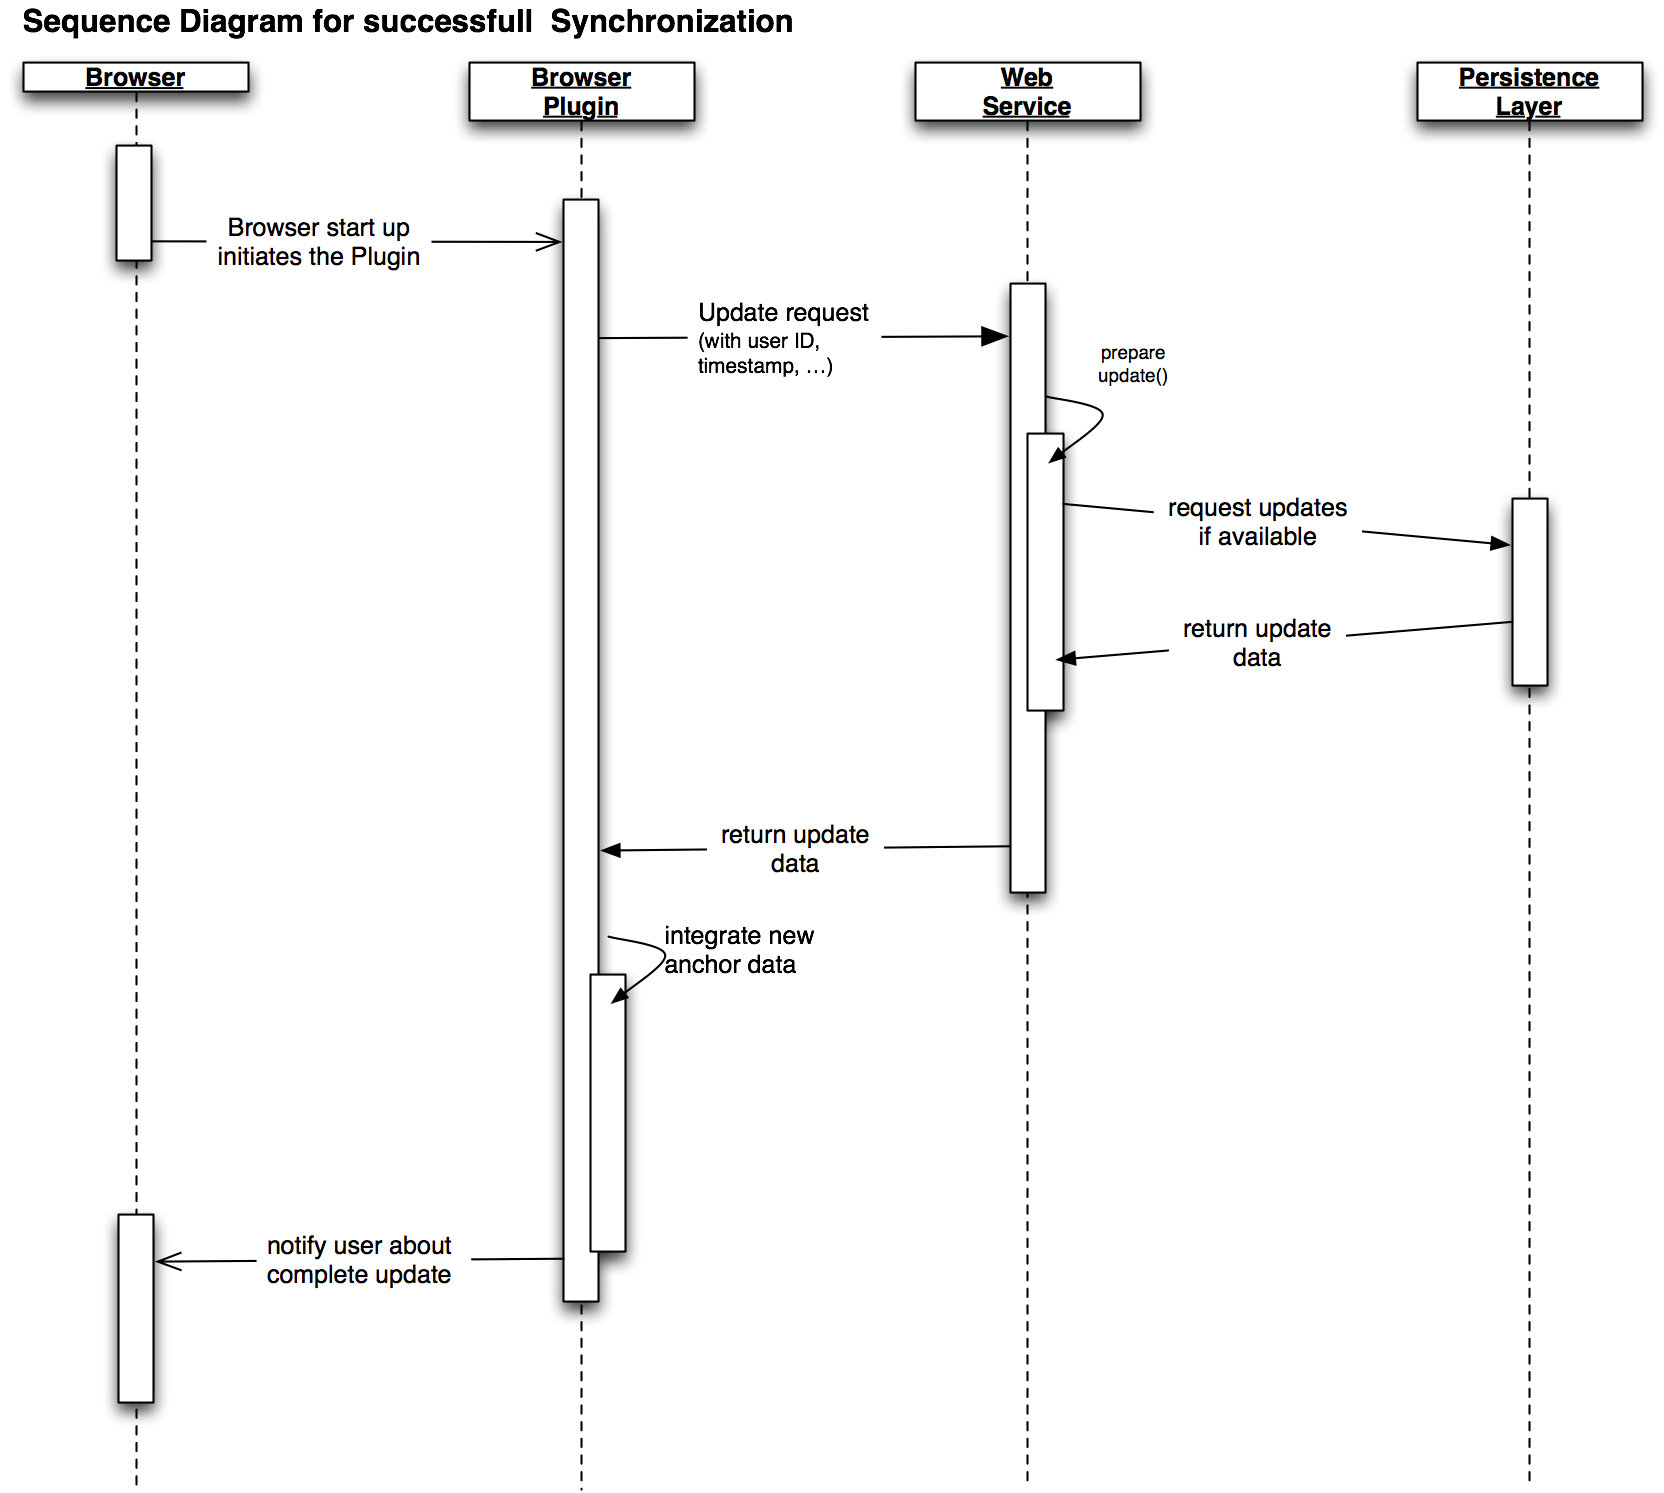
\includegraphics[width=13cm]{images/sequence-update.png}
		\caption{Sequence diagram for a successful plugin update}
		\label{sequence-update}
\end{figure} 

\subsubsection{Matching Procedure}
When we use the term matching procedure it means that existing anchors are visualized to the user. Before every matching procedure we assume that an update is triggered to ensure that the newest data is being used. 

Beyond the update procedure there is no need communicate with the server. When the user opens a new URL it triggers the matching procedure. The plugin searches its local content whether there are some anchors for this URL. In a positive case (see Figure \ref{sequence-matching-process}) the content is visualized to the browser view. 

At this point Alice would receive nothing from the plugin since no anchors exist for \verb+www.cal.google.com+. 

The way how anchors are retrieved from the plugin is quite similar how it is done at the back end. The major difference is that we do not use any time stamps at this time. There is no need for that since we assume everything is up to date after the update procedure. 

\begin{figure}\centering
		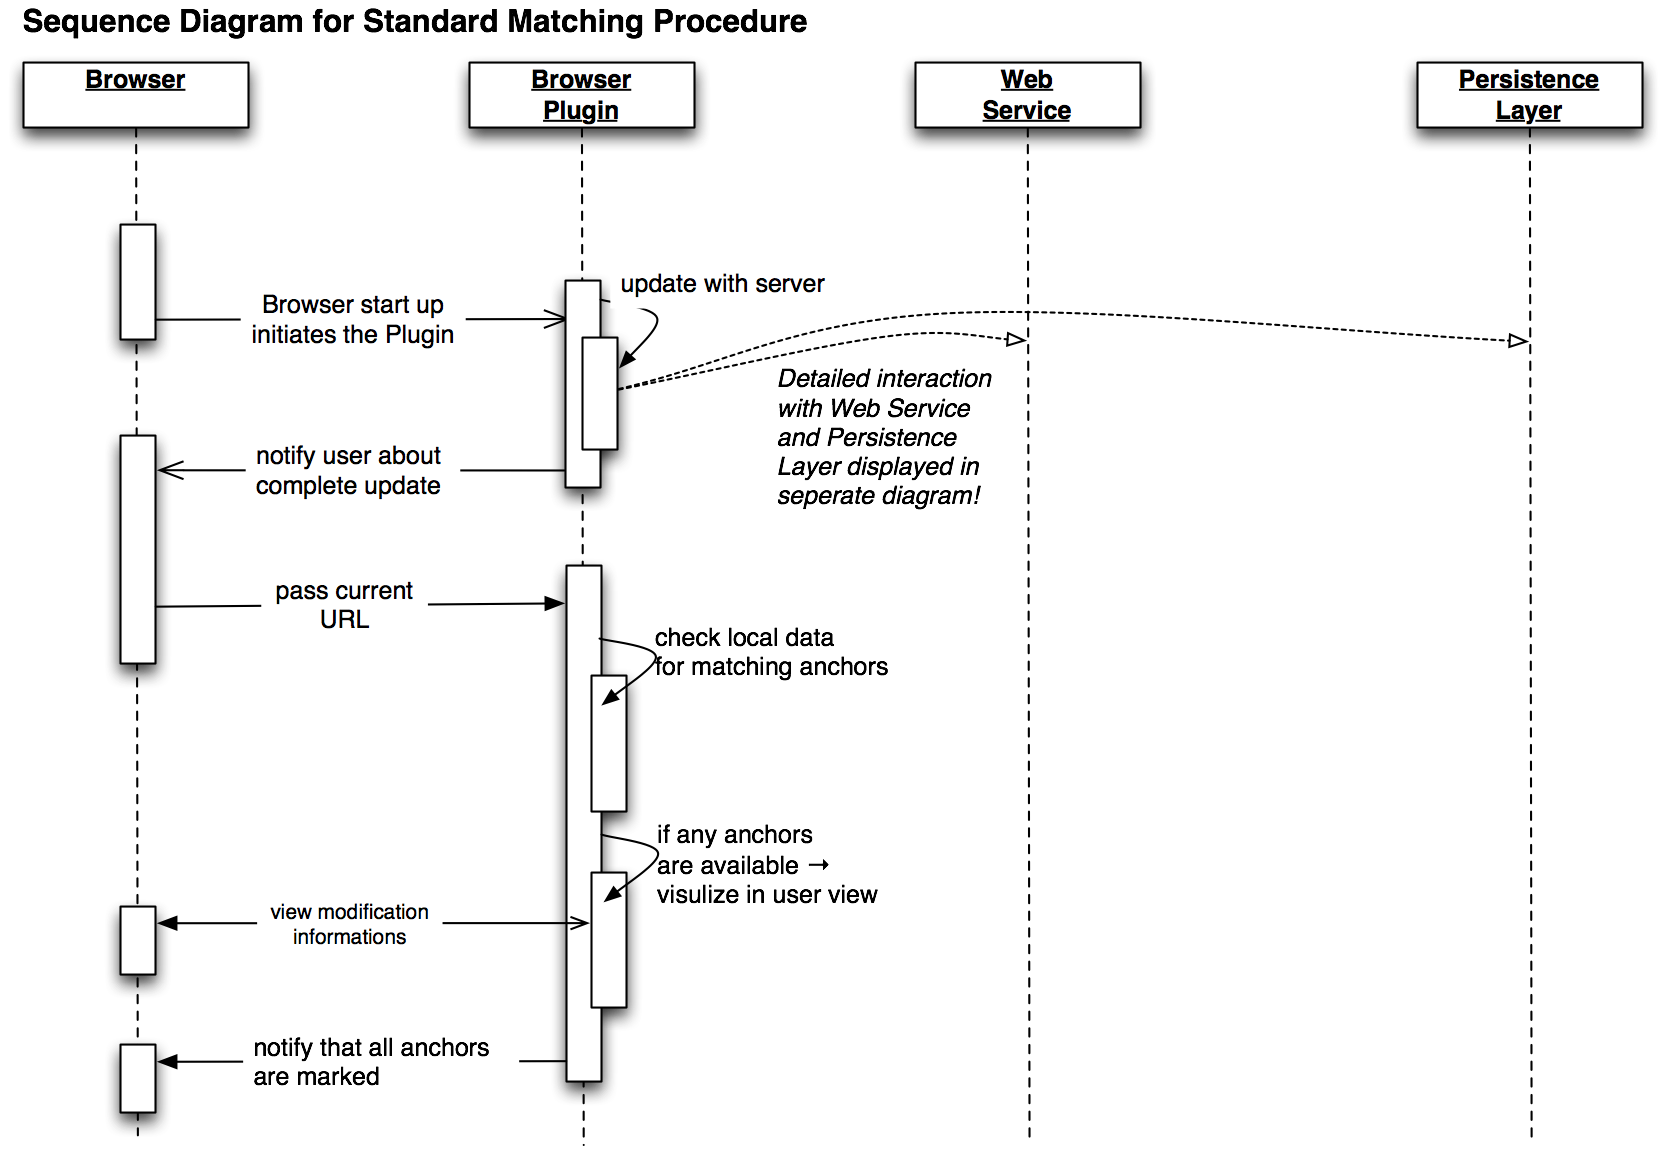
\includegraphics[width=13cm]{images/sequence-matching-process.png}
		\caption{Sequence diagram for a standard matching procedure}
		\label{sequence-matching-process}
\end{figure} 

\subsubsection{Scenario Execution}
Now that we learned about the two sub-procedures we are able to start with the actual scenario. First step is going to be that Alice weaves a comment box to an appointment: 

\begin{figure}\centering
	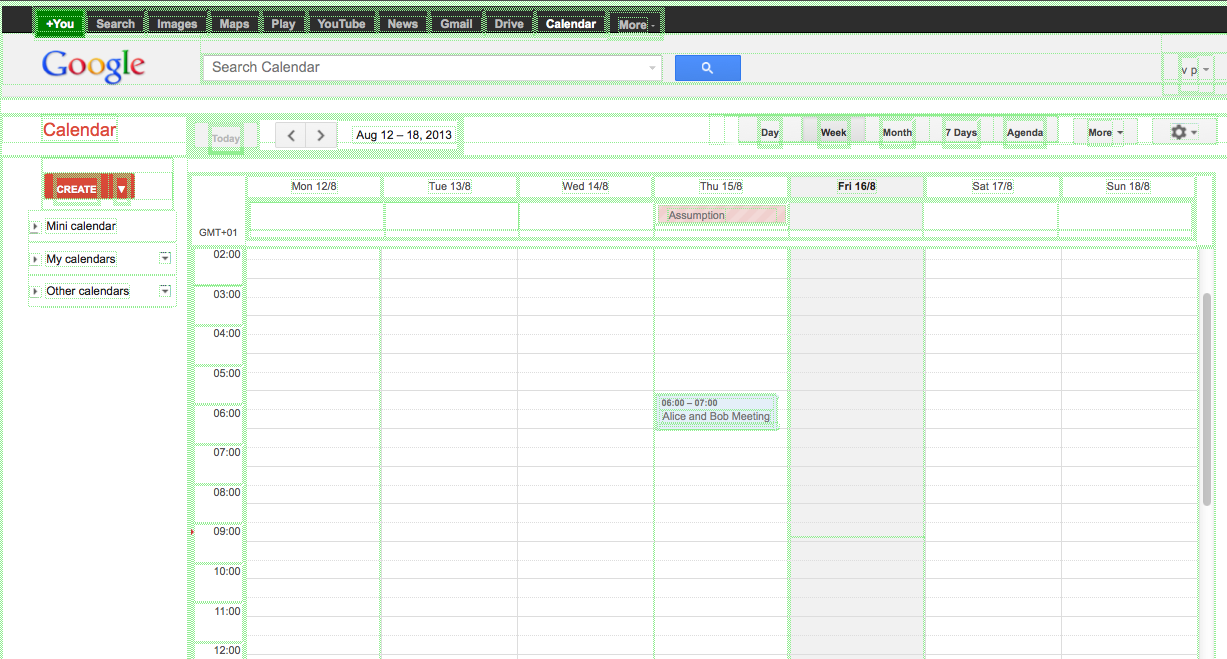
\includegraphics[width=13cm]{images/gcal-marking-mode.png}
\caption{Activated Marking Mode}
\label{gcal-marking-mode}
\end{figure}

Alice enters \verb+www.cal.google.com+ which first of all triggers an update. Afterwards potentially new anchors would be displayed in the browser - which is not the case right now. 
Now Alice is able to mark an appointment (see Figure \ref{gcal-marking-mode}). By clicking an element she appends a comment box. 
In the background the plugin runs the script (or scripts) that are related to the URL to define an identifier for the element. 
Using this identifier, the content-data for the comment box and the current URL the plugin creates a message in JSON format and passes it to the server. 

The content for the comment box in this case is just a link. We use an external comment system that is injected as HTML code (see Figure \ref{gcal-commentbox}). Where or how exactly this comment box is defined, is not relevant to our matters.

\begin{figure}\centering
	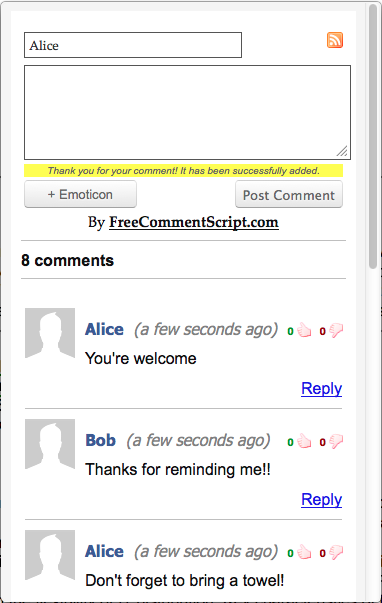
\includegraphics[width=4cm]{images/gcal-commentbox.png}
\caption{Comment Box}
\label{gcal-commentbox}
\end{figure}

For our example the JSON file might look like:

\begin{lstlisting}[language=JavaScript]
{
	content-data='www.chatsystem.com/alice-apointment-17349',
	element-id='7234808234088023480',
	current-url='www.cal.google.com'
}
\end{lstlisting}

The message is passed as an authenticated POST Rest request. The web service performs some checks before the anchor is persisted. For instance it could be the case that there is already an anchor for exactly this element (because an other user created one in the meantime or the element identifier is not unique in this context). 

In our scene everything works out fine and the web service persists the new anchor in the PostgreSQL database. The web service returns a positive status code to the plugin. This again triggers the previously discussed update and matching procedure. Alice sees her comment box attached to the appointment after it is guaranteed to be persisted on the server. It is not possible that the plugin creates locally new anchors that do not exist on the server. 

\begin{figure}\centering
		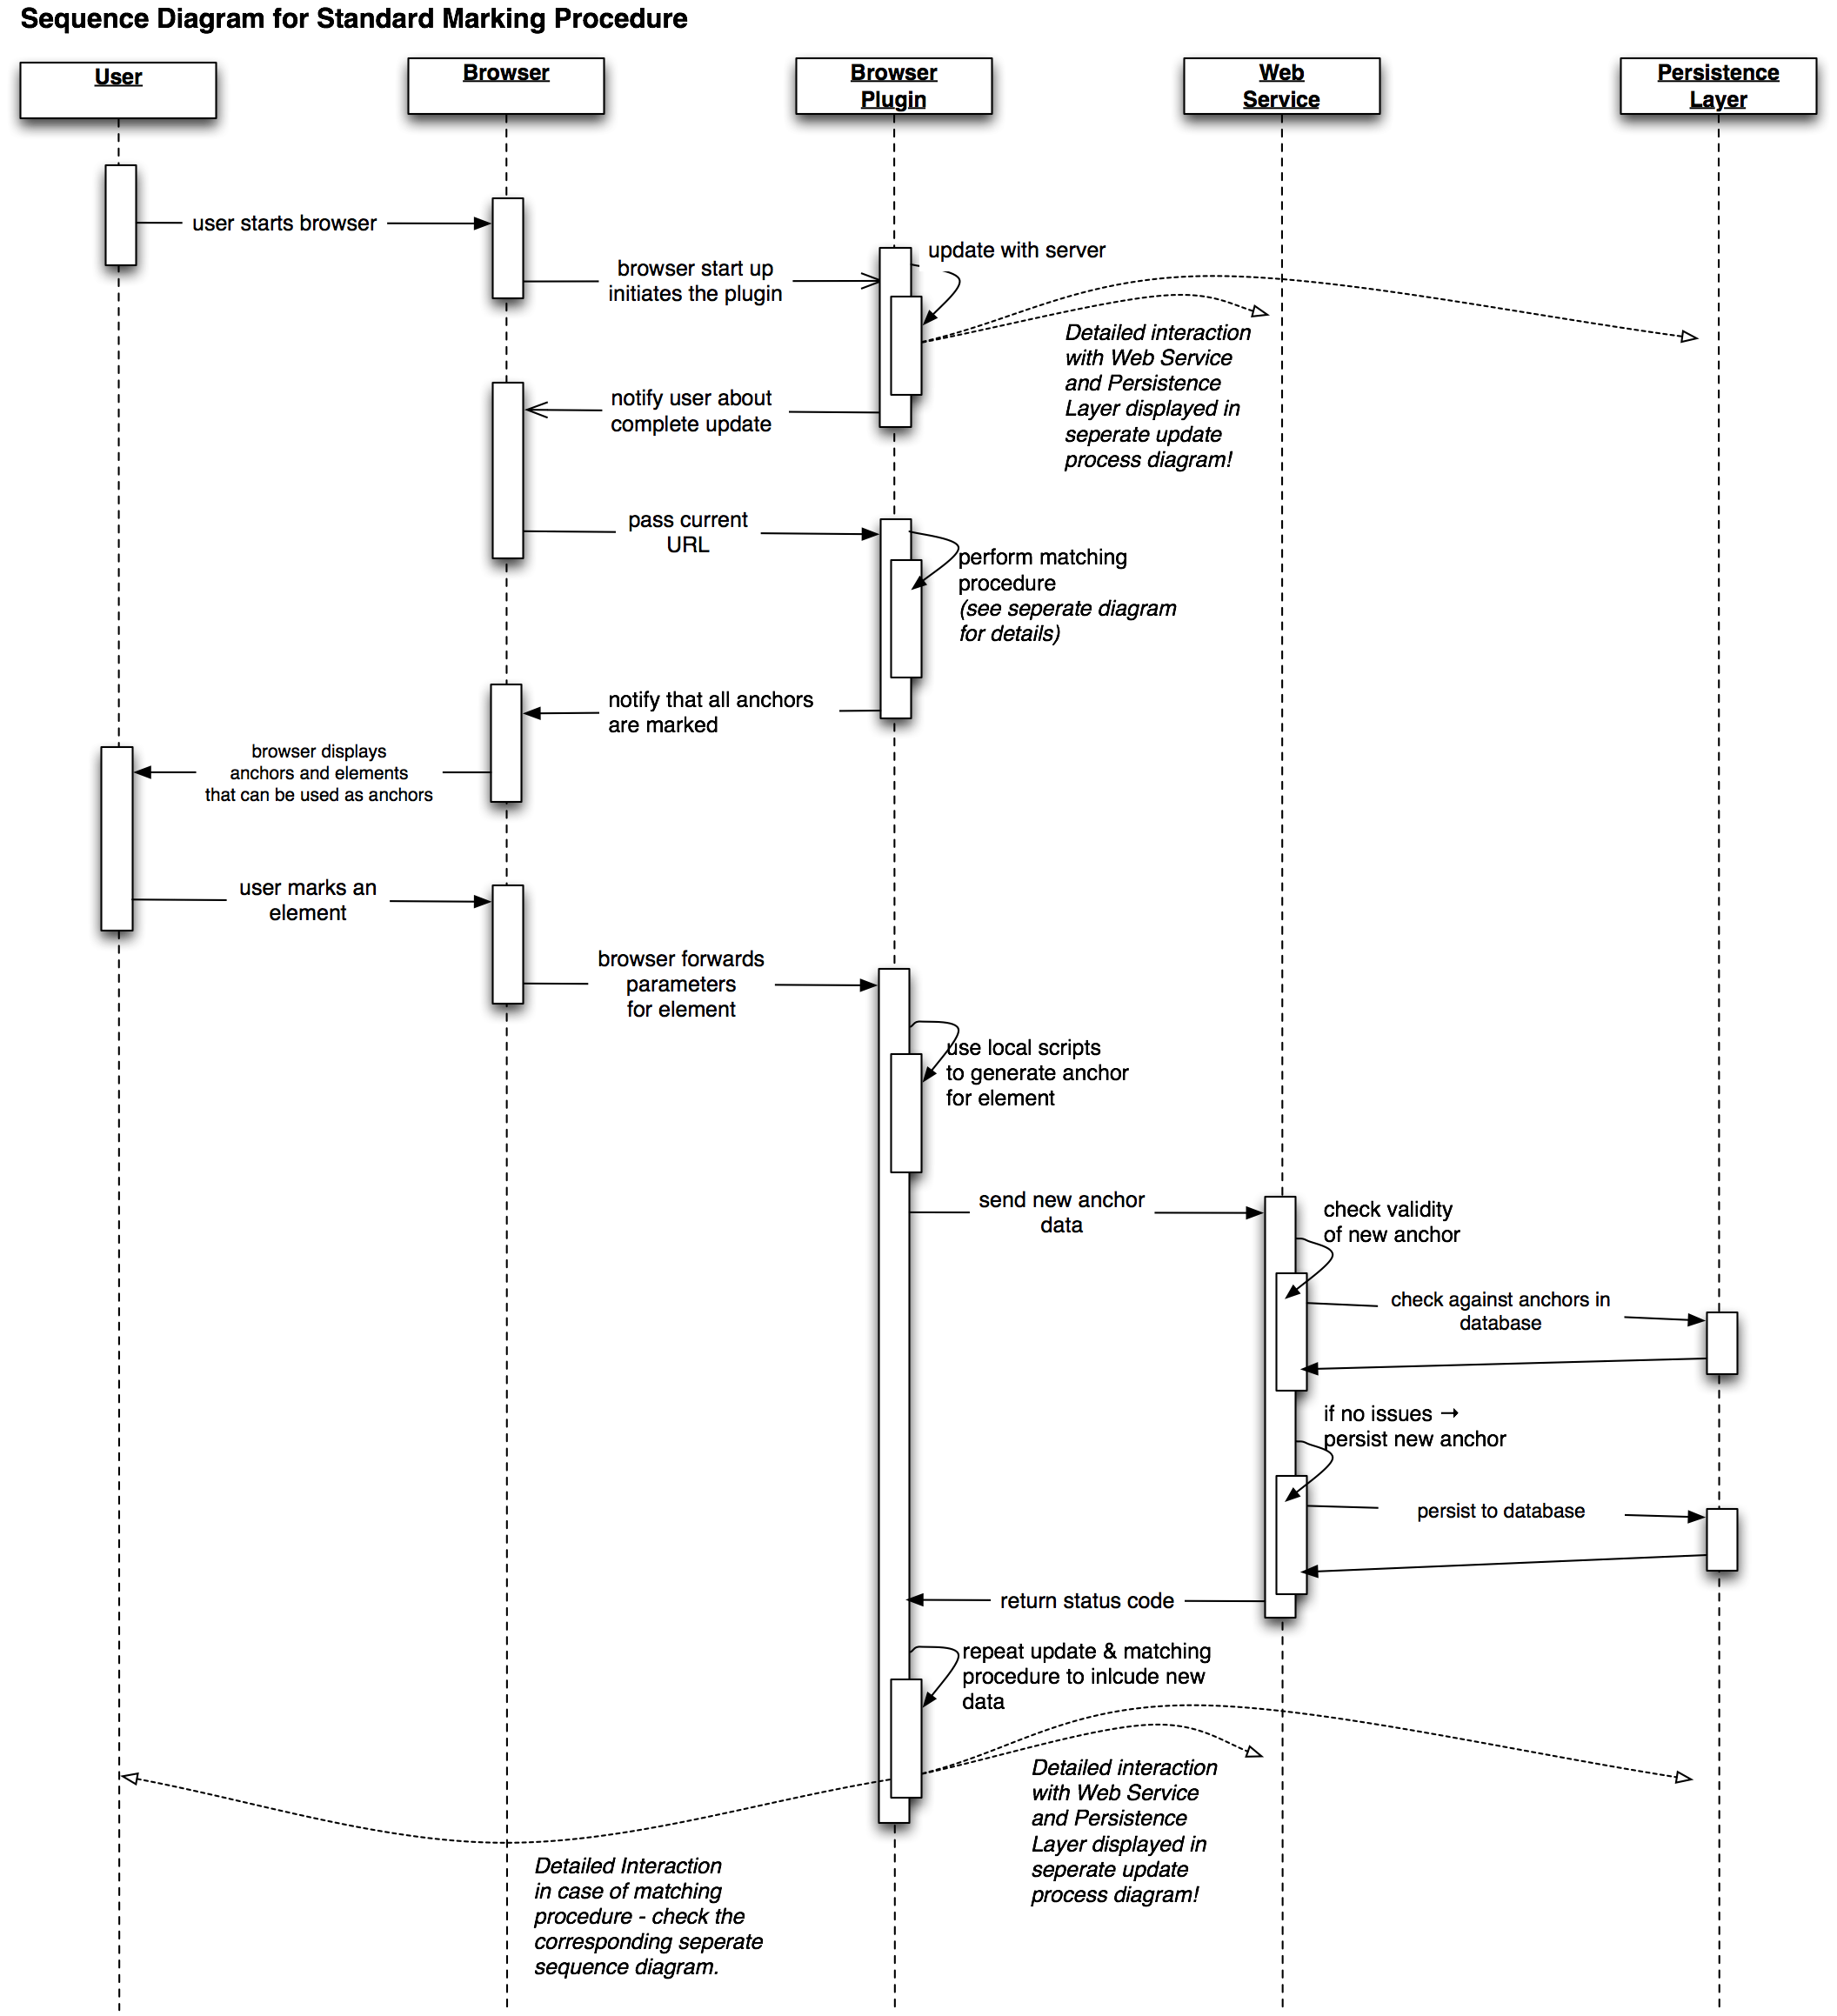
\includegraphics[width=13cm]{images/sequence-marking-process.png}
		\caption{Sequence diagram for standard marking procedure}
		\label{sequence-marking-process}
\end{figure} 

Finally it is possible for Alice to use the comment box. This step is very simple. As we already mentioned the comment box is an external service that is only injected by a link into our system. Therefore Alice can add a comment without any consequences to our system at all.

Now it is Bobs turn. This process is quite similar and partially redundant to what happened when Alice created the anchor. For that reason we do not go into detail like we did for the first step.

\begin{figure}\centering
	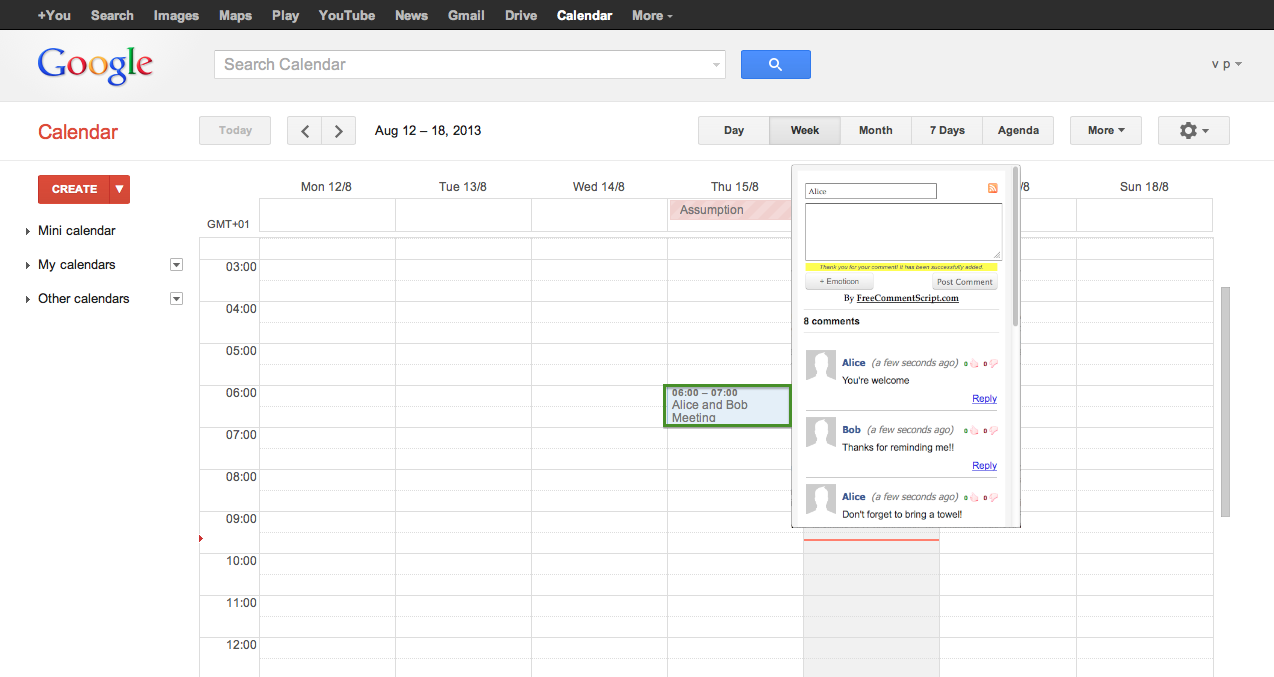
\includegraphics[width=13cm]{images/gcal-combined.png}
\caption{Comment box woven into Google Calendar}
\label{gcal-combined}
\end{figure}

Bob opens the Google Calendar website, which triggers the update and matching procedure for this URL. Since there is an existing anchor now - Bob's plugin receives the data for displaying the comment box entered by Alice (see Figure \ref{gcal-combined}). 

The last two steps are getting more interesting again. We basically simulate a evolution of a website that destroys our anchor mechanism. That can happen very easily depending on the type of script we are using or how fast the webpage evolves, but this issue is discussed more deeply in the coming Section \refname{sowe-assessment} \ref{sowe-assessment}. What we do is to modify the element identifier directly in the database. This way it becomes impossible to match this anchor for the given URL. 

So Alice visits her calendar to check whether Bob has reacted to her reminder. Again an update and matching procedure is started. The update works seamlessly, but an error occurs while the matching progresses. The plugin runs the script to determine the element that belongs to the element id - but with no success. 

For that case the plugin enables Alice to re-link the content to the correct element or as in this case - appointment. The plugin performs the two following steps:
\begin{enumerate}
	\item Create a new anchor element, that is basically a copy to the old one but with a correct element-id. This step is identical to the above described procedure when Alice weaved the comment box into an appointment the first time. 
	\item  Additionally to the first step, we need to remove the broken anchor from the server. This is done by sending a remove Rest request to the server including the old element identifier. 
\end{enumerate} 
After those steps are finished, it is necessary to run the update and matching procedures again. Now Alice and Bob are able once again to use the comment box. 

Re-linking an anchor does not necessarily has to be due to an error or web page evolution. For instance, if Bob changed the time of the appointment - the anchor would not work either. In this case a re-link would solve the problem as well.

\newpage

\subsection{Social Weaver Assessment}\label{sowe-assessment}
In the following we analyze how good Social Weaver works in several real scenario cases. Since it is developed as a proof-by-concept prototype, a general support for all web sites or web application is out of reach. Anyway the script support allows us to reach at least some flexibility even for complex web sites. The testing range covers static, dynamic and Web 2.0 web sites. A tabular overview is shown in Figure \ref{assessments-results}. We distinguish some criteria:

\begin{figure}\centering
		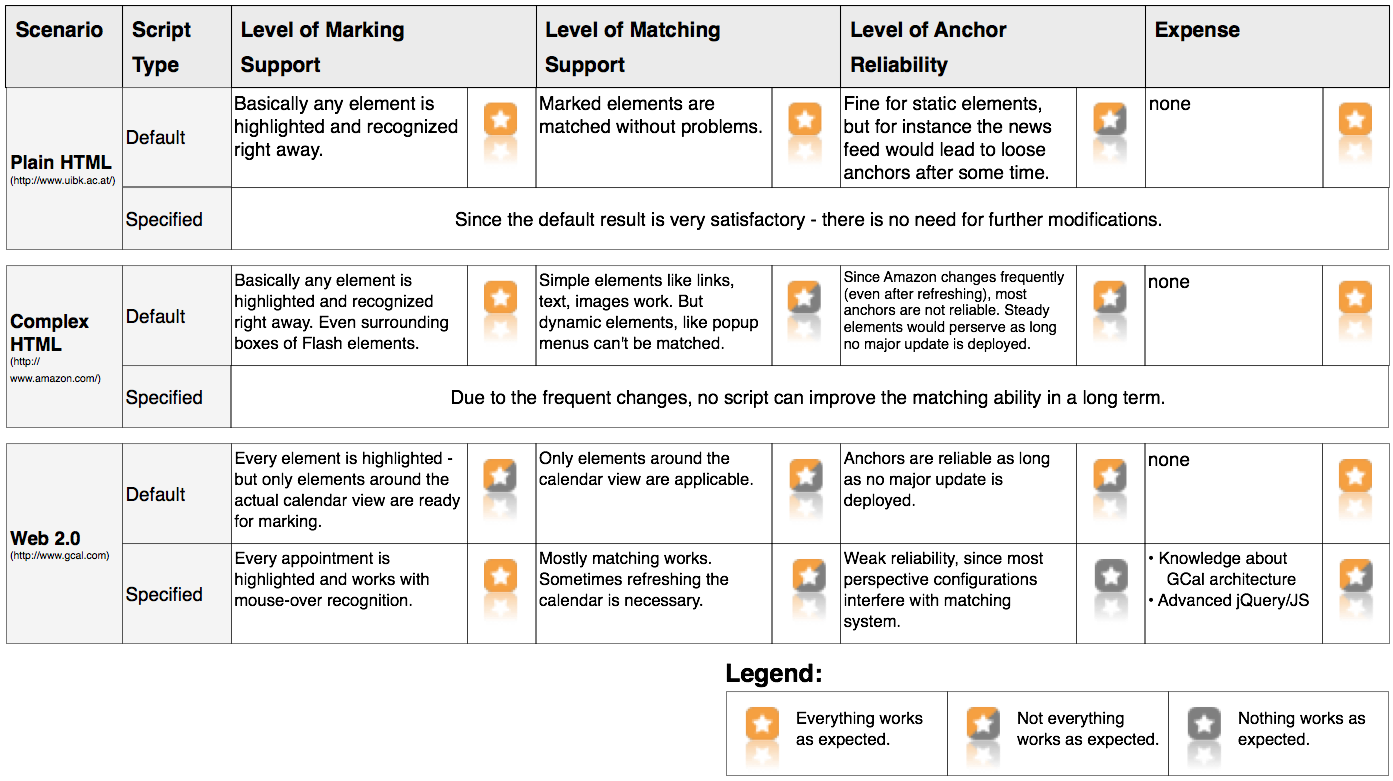
\includegraphics[height=0.7\textwidth, angle=90]{images/assessments-results.png}
		\caption{Assessment results for the Social Weaver prototype in differen scenarios}
		\label{assessments-results}
\end{figure} 

\begin{itemize}
	\item Level of Marking Support \\
	This criterion is the ability of the plugin to recognize elements in a web view. This means first of all that all relevant elements should be recognized. The best case would that elements like advertisements or scrolling bars would be left out. Still all buttons, form elements and similar elements would be spotted. This criterion is not purely objective since relevant elements may differ for each user.
	
	\item Level of Matching Support \\	
	Matching Support describes the ability of the plugin to find element that were previously marked. Even though this is at least as important as the Marking Support, there is no guarantee that matching is handled equally well as marking. For instance, if we match an element only by its path in the DOM tree; This path might be ambiguous to another element. In this case our social element would be weaved into the wrong place. We consider this as the worst case - even worse as if no element could have been matched.
 
	\item Level of Anchor Reliability \\
	Anchor Reliability can be seen as part of the matching criterion. But with reliability we refer to the time relevant aspect. With the evolution of a web page, our anchor information might become obsolete. The chance for this to happen is increasing with time. News pages are the best example for a very fast evolution. An anchor attached to an article on the front page would not last more than a couple of days. But even on such a dynamic web page there mostly are elements that are more reliable (e.g. the search column or navigation bars). 
	
	This criterion should evaluate how probably it is that anchors outlast time. 
	
	\item Expense \\
	Expense in this context means how much effort has been used to give support for the tested environment. The extent of the script itself and an appraisal, about how tricky the construction of the script is, whether just standard procedure has been used or if it was necessary to insert some hacks. 
\end{itemize}

\subsubsection{Script Types}
For each scenario we consider two script types. One is the simple default script and the other one a specified script, based on the current scenario.

\begin{figure}\centering
\begin{lstlisting}
{
    "rules": [
        {
            "doc_location": "document.location.toString()"
        },
        {
            "element_content": "matchedElement.text()"
        }
    ]
}
\end{lstlisting}
		\caption{Default script JSON code}
		\label{default-script-code}
\end{figure} 

\paragraph{Default Script}\mbox{}\\
The default script (see Figure \ref{default-script-code}) is the quite simple combination of the document location combined with the textual content of the element. Even though this approach has many drawbacks and is no general solution at all, it works often with satisfactory results in practice. There is an easy explanation for that: When an element is clearly identified by the user, this is mostly the case because of some textual information. At the same time this information is as well the HTML content of the element. 

In the following the default script is always the same JSON rule list as seen in Figure \ref{default-script-code}. 

\paragraph{Specified Script}\mbox{}\\
The specified script is related to the according scenario. In cases where the default script does not suffice, it might be possible to improve the Social Weaving functionality with a specified script. The author of such a script requires knowledge about the environment. When discussing the scenarios, it becomes obvious when a specified script might come in useful. 

\subsubsection{Scenario: Plain HTML}
We start slow with an (predominantly) static HTML environment; the web page for the University of Innsbruck (http://www.uibk.ac.at). Today even simple web pages contain technologies like Ajax, PHP or JavaScript, which technically does not count as static anymore. But in our context it the frequency of changes is more important. 

\begin{figure}\centering
		
\includegraphics[width=13cm]{images/3d-uibk.png}
		\caption{3D representation of \url{http://www.uibk.ac.at/}}
		\label{3d-uibk}
\end{figure} 

The following steps are performed for this scenario:
\begin{enumerate}
\item Annotate one link and one image
\item Navigate somewhere else, or quit the browser
\item Return to the starting position
\item Check whether the marks are visible
\item Check whether the annotations are still intact
\end{enumerate}
\paragraph{Default Script: University of Innsbruck}\mbox{}\\
\begin{figure}\centering
		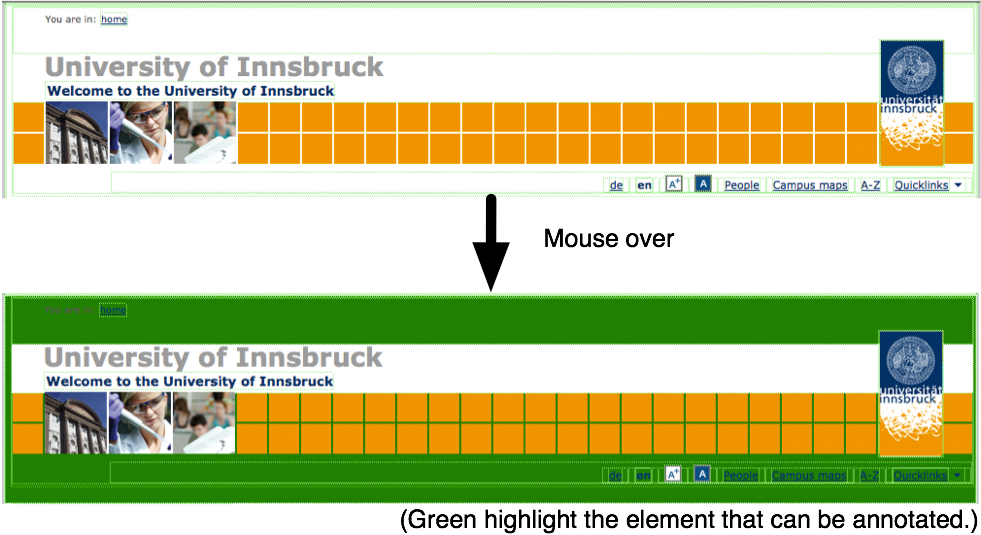
\includegraphics[width=8cm]{images/bad-example-backgroundbox.png}
		\caption{Bad example for marking elements.}
		\label{bad-example-backgroundbox}
\end{figure} 
\begin{tabular}{|p{0.2\textwidth}| p{0.8\textwidth} |}
\hline 
Level of Marking Support & Once the marking mode is active, every element is highlighted correctly. Moving the cursor over the elements precisely chooses the element beneath it. Only drawback is, that some background boxes are selectable, which is not harmful, but as well not useful (see Figure: \ref{bad-example-backgroundbox}).\\ 
\hline 
Level of Matching Support & Either the link as well the image are matched after re-navigating to the web site. \\ 
\hline 
Level of Anchor Reliability & This scenario is mostly static. Except for a news feed section, the anchors would remain persistent, as long no greater changes happen to the web site. \\ 
\hline 
Expense & None \\ 
\hline 
Conclusion & The results with the default script for the mostly static web site are quite satisfactory. All the expected functionality is provided. \\ 
\hline 
\end{tabular} 
\paragraph{Specified Script: University of Innsbruck}\mbox{}\\
The default script fulfills all the requirements, therefore we have no need to improve the Social Weaving functionality with a specified script. 

\subsubsection{Scenario: Complex HTML}
In this case we test Social Weaver on the start page of Amazon. The purpose is to review a dynamic web site and to show the immense disadvantage with high frequency changes. A desirable feature would be to annotate a purchasable item, that would be matched in any environment. This nevertheless exceeds the basic idea of Social Weaving; but would be possible with a proper specified script. 

\begin{figure}\centering
		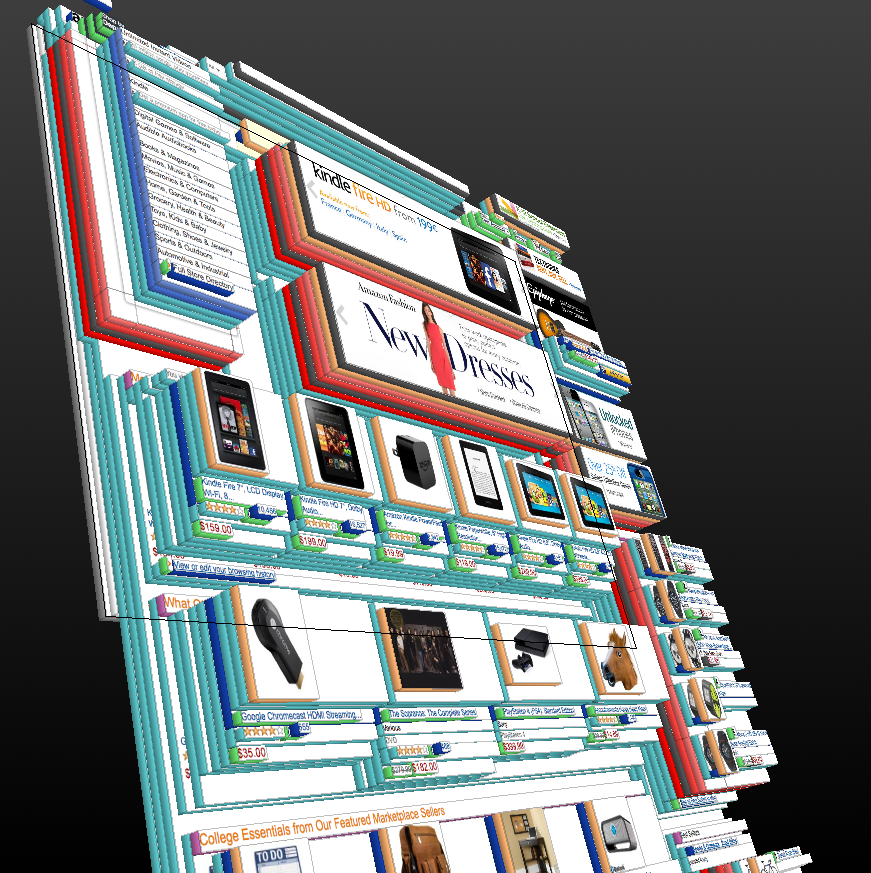
\includegraphics[width=13cm]{images/3d-amazon.png}
		\caption{3D representation of \url{http://www.amazon.com/}}
		\label{3d-amazon}
\end{figure} 

The following steps are performed for this scenario:
\begin{enumerate}
\item Annotate one link, one dynamic element (like popup menu) and a Flash window
\item Navigate somewhere else, or quit the browser
\item Return to the starting position
\item Check whether the marks are visible
\item Check whether the annotations are still intact
\end{enumerate}

\paragraph{Default Script: Amazon}\mbox{}\\
\begin{tabular}{|p{0.2\textwidth}| p{0.8\textwidth} |}
\hline 
Level of Marking Support & All elements are highlighted, but there are problems at some points with the mouse-over recognition.  The reason for this issue, it that mouse-over recognition is as well used by the web site itself. The plugin and the web site use the same JavaScript methods, which obviously results in interference. Despite this problem most elements act naturally.\\ 
\hline 
Level of Matching Support & Success of element matching depends on the element type. The annotated link is matched correctly, but the dynamic and Flash element fail in most cases. Even worse than that, is the unpredictability of whether matching will work or not. Extended knowledge about the web site is necessary to address such problems. \\ 
\hline 
Level of Anchor Reliability & We choose Amazon as a worst case scenario for Social Weaving, since the updates on the web site are very frequent. Already refreshing the browser leads to a quite different view, since the sale item proposals might be adjusted to user cookies. Most of the possible elements are not fitting for becoming an anchor. \\ 
\hline 
Expense & None\\ 
\hline 
Conclusion & Amazon is intentionally chosen to show the weakest side of the prototype. Frequent updates and many dynamic elements make it very hard to provide full Social Weaving support. 

Furthermore it requires a deep knowledge of the web site architecture for designing a good script. Besides the script needs to follow different goals. When we talk about Social Weaving, we assume a view where anything relevant can be annotated. In the case of Amazon, this assumption does not hold. An option is to focus on the sale items and match those across navigation. Alternatively only static elements are valid for annotations. \\ 
\hline 
\end{tabular} 
\paragraph{Specified Script: Amazon}\mbox{}\\
It is impossible to provide a script that overcomes frequent changes on the web site. As mentioned in the previous conclusion, a script for different goals is an option - but this approach goes beyond this thesis. 

\subsubsection{Scenario: Web 2.0}
In this scenario we deal with the Web 2.0 web application Google Calendar (GCal). But first it's specified what Web 2.0 actually means.

\paragraph{What is Web 2.0}\mbox{}\\
\begin{figure}\centering
		
\includegraphics[width=10cm]{images/web2.png}
		\caption{web2}
		\label{Web 2.0 tag cloud - a common Web 2.0 feature itself.}
\end{figure} 

Actually there is not strict definition for the term Web 2.0. It seems that it was coined by Tim O'Reilly at the O'Reilly Media Web 2.0 conference in late 2004 (\cite{o2005web}). A very brief way to describe the difference between Web 2.0 and the web that existed beforehand is \emph{read and write web}. Basically, web services where the user has the possibility to modify the content, should be seen as Web 2.0. 

The most popular representatives for Web 2.0 are platforms such as Facebook, Twitter and Youtube.

\paragraph{Scenario Description}\mbox{}\\
Finally we test Social Weaver on an actual Web 2.0 scenario, more specifically we annotate an appointment within GCal. Although the calendar view might seem minimalistic and simple from the users perspective, the architecture beneath the visible layer is very complex. Compare the 3D structure of Figure \ref{3d-gcal} to the other representation of our previous scenarios, shown in Figure \ref{3d-uibk} and \ref{3d-amazon}. GCal has the most layers (as long as we do not count the advertisement layers at Amazon, which do not really affect the complexity of the architecture). The reason for the complexity in GCal is the flexibility for different calendar views. Perspectives for single days or  weeks are supported. The relation and positioning of the appointments requires many dynamic shortcuts. Without question this is great for the application usage, but not welcoming for Social Weaving. 

\begin{figure}\centering
		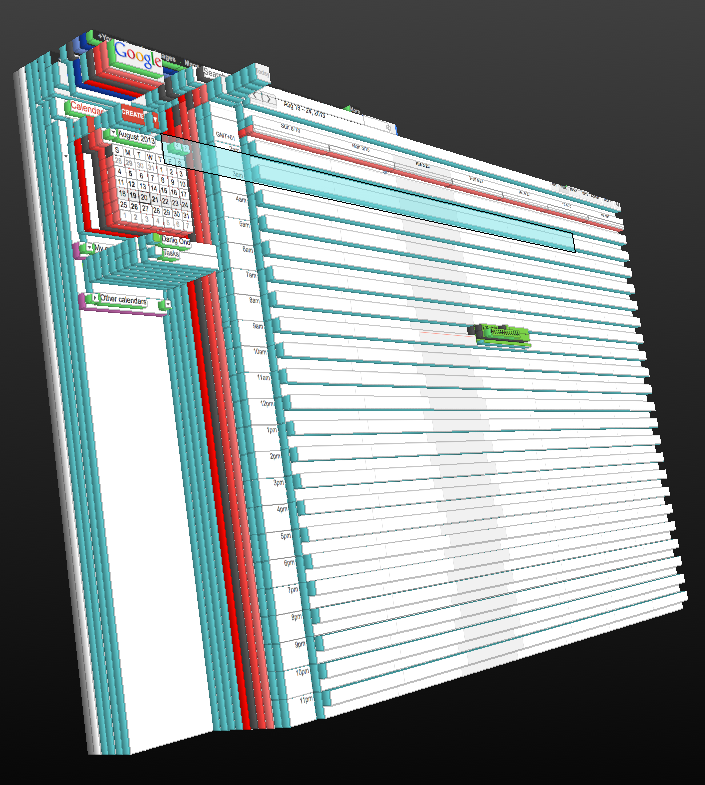
\includegraphics[width=13cm]{images/3d-gcal.png}
		\caption{3D representation of \url{https://www.google.com/calendar/}}
		\label{3d-gcal}
\end{figure} 

This time we perform the following steps for the scenario:

\begin{enumerate}
\item Annotate one appointment and one element not in the actual calendar view
\item Navigate somewhere else, or quit the browser
\item Return to the starting position
\item Check whether the marks are visible
\item Check whether the annotations are still intact
\end{enumerate}


\paragraph{Default Script: Google Calendar}\mbox{}\\
\begin{tabular}{|p{0.2\textwidth}| p{0.8\textwidth} |}
\hline 
Level of Marking Support & All elements are highlighted correctly, but already the mouse-over recognition only works for elements around the calendar view. Marking is, as well, only possible for those elements. Interaction with appointments is not possible.\\ 
\hline 
Level of Matching Support & The elements that can be marked, also are matched correctly. Since this only applies to part of the environment (and moreover the less important, because we want to annotate appointments), this should be considered as failure. \\ 
\hline 
Level of Anchor Reliability & The reliability depends on the marked element. Some fields (like dates or calendar names) might change with a differently configured perspective, which would break the anchor connection.  \\ 
\hline 
Expense & None \\ 
\hline 
Conclusion & It is not surprising that the default script does not properly work in that case. Obviously there is need for a specified script.\\ 
\hline 
\end{tabular} 

\paragraph{Specified Script: Google Calendar}\mbox{}\\
The goal of the specified script (see Figure \ref{gcal-spec-script}) is to annotate appointments. Since GCal does not use any visible unique identifiers for appointments across user sessions, we must use some workarounds. What the script basically does, it to gather some parameters that identify the appointment uniquely. Each rule has its own purpose:

\begin{description}
\item[doc\_location] Simply checks the URL of the current document. We use this as well in the default script. 
\item[appointment\_title] Starting from the user-clicked element we step down, child by child, until to the \emph{span} field. The \emph{innerHTML} is the title of the appointment. 
\item[appointment\_time] Same starting point as for \emph{appointment\_title}, but a slightly different step-down path, leads to the text value, that determines the time. Additionally we filter out further information in that area (like Reminders). 
\item[appointment\_date\_1] This rule moves from the user-clicked element up, parent by parent, until \emph{td} is reached. The first child of this parent contains an \emph{id} that denotes the column, the appointment is in. We need this rule as a part to recognize the date.

\item[appointment\_date\_2] GCal maintains a \emph{from-to-date} field. We retrieve this, using jQuery and add it as parameter to our anchor. 
\end{description}

The first three rules are straightforward, but the last two rules, that are responsible for the date, require some explanation. The reason for this complicated way, is that GCal maintains the week-view layer and the appointments-view layer at different levels. This means that there is no direct in-code relation to what date the appointment actually takes place. The position is set at the server side. So what we need to do, it to check the position, or column, of the appointment (see rule \emph{appointment\_date\_1}). Additionally we combine it with the information about the date range, the week is located in (see rule \emph{appointment\_date\_2}). 

Keep in mind that this script only supports the standard week view. Switching, for example, to single-day perspective is not supported. There are several more factors that would interfere with script. Different timezones would require a more complex approach and many more rules. Due to the fact that we use plain strings as parameters, even time representations like 12h or 24h are problematic.

\begin{figure}\centering
\begin{lstlisting}
{
    "rules": [
        {
            "doc_location": "document.location.toString()"
        },
        {
            "appointment_title": "matchedElement.filter('dl > dd > span').innerHTML"
        },
        {
            "appointment_time": "matchedElement.filter('dl > dt').filter('i').innerHTML"
        },
        {
            "appointment_date_1": "matchedElement.parentsUntil('td').children(':firstChild').attr('id')"
        },
        {
            "appointment_date_2": "$('.currentDate:2').innerHTML"
        }
    ]
}
\end{lstlisting}
\caption{Specified script for Google Calendar}
\label{gcal-spec-script}
\end{figure} 

\begin{tabular}{|p{0.2\textwidth}| p{0.8\textwidth} |}
\hline 
Level of Marking Support & Correct elements are highlighted and work with mouse-over recognition. With the specified script only appointment fields are supported.\\ 
\hline 
Level of Matching Support & Mostly the matching works correctly. Sometimes a refresh is necessary to re-run the matching procedure. \\ 
\hline 
Level of Anchor Reliability & The reliability is to be expected very unstable. There are many configuration options the user can make to modify the calendar perspective. Even minor changes, like having Monday or Sunday as the first day of the week, leads to unwelcome results. \\ 
\hline 
Expense & Knowledge about the GCal architecture and advanced usage of jQuery/JavaScript \\ 
\hline 
Conclusion & This scenario shows, that it's possible to reach flexible functionality with specific scripts. But on the other hand, the tricky process and outlay, make clear, that good support needs effort. To support a Social Weaving level for GCal, such that normal users could use it without any trouble, would require a lot of exception handling and multiple scripts for different perspectives. \\ 
\hline 
\end{tabular} 


